\begin{figure}
    \centering
    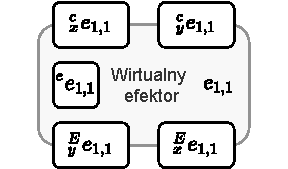
\includegraphics[width=0.75\columnwidth]{figures/ISR-ve-manip-model.pdf}
    \label{fig:model-vr-camera}
    \caption{Struktura ogólna wirtualnego efektora manipulatora sześciostopniowego}
\end{figure}

\begin{figure}
    \centering
    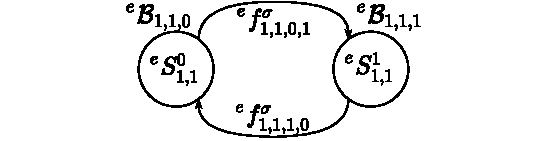
\includegraphics[width=\columnwidth]{figures/ISR-ve-manip-behaviours.pdf}
    \label{fig:zachowania-ve-manip}
    \caption{Automat zachowań wirtualnego efektora manipulatora sześciostopniowego}
\end{figure}

Efektor wirtualny manipulatora:
\begin{itemize}
    \item bufor wejściowy od podsystemu sterowania: pozycja pożądana,
    \item bufor wyjściowy do podsystemu sterowania: pozycja aktualna,
    \item bufor wejściowy od rzeczywistego efektora: aktualne położenie wałów silnika,
    \item bufor wyjściowy do rzeczywistego efektora: pożądana pozycja wałów silnika.
\end{itemize}


Zachowania:
\begin{itemize}
    \item ${}^{e}\mathcal{B}_{1,1,0}$ - idle,
    \item ${}^{e}\mathcal{B}_{1,1,1}$ - move.
\end{itemize}